\documentclass[11pt]{article}
\usepackage{arduino-uppgifter}

\newcommand{\mallurl}{https://wokwi.com/projects/357812594927244289}

% Figures subfolder
\graphicspath{{figures/}}

\begin{document}
\begin{center}
      \textbf{\huge{Arduino-övningar}}
      \huge{| MEKMEK01 v11}
\end{center}
\raggedright{}
\begin{center}
      \paddedfbox{
            Nedan kommer några ideer på övningar som kan göras med Arduino. Ni
            kommer att
            ha användning för kunskapen som krävs för att lösa dessa övningar i
            ert
            projektarbete senare i kursen.
      }
\end{center}

\section{Flera blinkande lampor}\label{sec:flera-lampor}
Skapa en krets med 5 lampor, där alla lampor blinkar samtidigt med ett jämnt
intervall, som nedan.
\begin{figure}[H]
      \animategraphics[autoplay, loop,
            width=0.8\linewidth]{1}{2-}{0}{2}
\end{figure}
\begin{figure}[H]
      \centering
      \begin{minipage}{0.4\textwidth}
            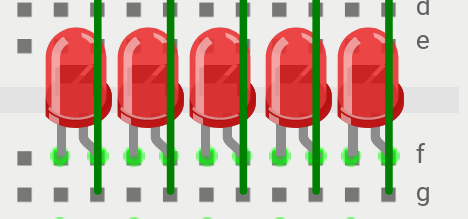
\includegraphics[width=\textwidth]{5led-low}
      \end{minipage}
      \begin{minipage}{0.4\textwidth}
            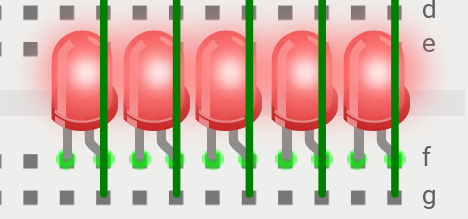
\includegraphics[width=\textwidth]{5led-high}
      \end{minipage}
\end{figure}

\section{Lampor blinkar en-efter-en}\label{sec:sekvensiell-blinkning}
Nu ska lamporna tändas en-efter-en i serie, som en ``mask'' som rör sig framåt.
När alla fem lampor har tänts ska alla släckas samtidigt och cykeln börja om.
\begin{figure}[H]
      \centering
      \begin{minipage}{0.3\textwidth}
            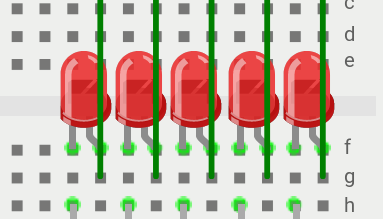
\includegraphics[width=\textwidth]{2-0}
      \end{minipage}
      \begin{minipage}{0.3\textwidth}
            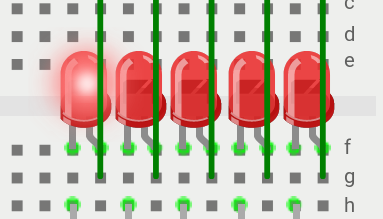
\includegraphics[width=\textwidth]{2-1}
      \end{minipage}
      \begin{minipage}{0.3\textwidth}
            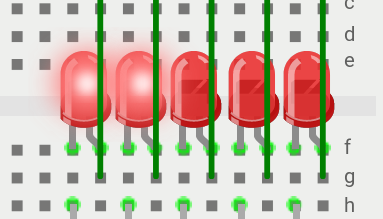
\includegraphics[width=\textwidth]{2-2}
      \end{minipage}
\end{figure}

\section{Multitasking: blinka olika lampor med olika intervall}
\paddedfbox{
      Uppgift \ref{sec:flera-lampor} och \ref{sec:sekvensiell-blinkning} kan
      lösas
      med \texttt{delay}. Ett problem med den lösningen är att Arduino inte kan
      göra
      något annat under tiden \texttt{delay} kallas på. Detta kan lösas, genom
      att
      använda \texttt{millis} och \texttt{if}-satser. Läs på om detta i
      \href{https://mek.samake.se/arduino/kompendium}{Arduino-kompendiet.}
}

Skapa en krets med två lampor, där den ena blinkar med ett intervall på 500ms
och den andra med ett intervall på 700ms.

\section{Ljusstyrka med PWM}\label{sec:pwm}
\paddedfbox{
      I uppgift \ref{sec:flera-lampor} och \ref{sec:sekvensiell-blinkning}
      används
      \texttt{digitalWrite} för att tända och släcka lampor. Detta är en
      binär (eller digital) funktion, det vill säga att lampan är antingen tänd
      eller släckt.
      Med funktionen \texttt{analogWrite} kan man istället styra ljusstyrkan på
      en lampa med hjälp av \texttt{PWM}. (Läs på om detta i
      \href{https://mek.samake.se/arduino/kompendium}{Arduino-kompendiet.})
}

Skapa en krets med en lampa som börjar med att lysa svagt, sedan ökar
ljusstyrkan
över två sekunder till max, och sedan minskar ljusstyrkan till svagt igen.
Detta repeteras om-och-om igen.

\section{Knapptrycksräknare}\label{sec:knapptrycksraknare}
\paddedfbox{
      Enpulsning är en teknik för att detektera när en signal precis går från
      låg
      till hög. Detta kan användas för att exempelvis räkna antalet gånger en
      knapp har tryckts. Läs på om detta i
      \href{https://mek.samake.se/arduino/kompendium}{Arduino-kompendiet.}
}

Skapa en krets med en knapp. När knappen trycks in ska en räknare öka med 1,
och räknarens värde ska skrivas ut i terminalen.

\subsection{Utökning av knapptrycksräknare}\label{sec:utokning}
Utöka kretsen från \ref{sec:knapptrycksraknare} genom att lägga till en
reset-knapp, och en minus-knapp. När reset-knappen trycks in ska räknaren
återställas till 0, och när minus-knappen trycks in ska räknaren minska med 1.

\vspace{4em}\hrule
\section*{Extra-uppgifter}
\paddedfbox{
      Dessa uppgifter är lite mer avancerade och är inte nödvändiga för att
      klara av projektet.
}

\section{Automatisk binär räknare}\label{sec:binar-raknare}
Skapa en krets med 4 lampor som räknar i binära tal. Räknaren kommer alltså att
kunna visa talen 0--15. När räknaren når 15 ska den börja om från 0. Räknaren
ska räkna upp med ett intervall på 1 sekund.

\section{Manuell binär räknare}\label{sec:manuell-binar-raknare}
Utöka kretsen från \ref{sec:binar-raknare} genom att lägga till två knappar.
Den ena knappen ska göra så att räknaren ökar med 1, och den andra knappen ska
göra så att räknaren minskar med 1.

\end{document}